\chapter{Východiská}\label{chap:vychodiska}
V tejto kapitole je cieľom poskytnúť prehľad základným pojmom a postupov pri tvorbe verifikačného 
nástroja pre programovaní jazyk UNITY. Predpokladá sa znalosť Kripkeho štruktúry a sémantiky \cite{br11}.

\section{UNITY}

UNITY vychádza z knihy Parallel Program Design - A Foundation, v ktorej bol UNITY popísaný a 
navrhnutý autormi K. Mali Chandy a Jayadev Misra z University of Texas. Je to teoretický jazyk, 
ktorý sa zameriava na to \textbf{čo}, namiesto toho \textbf{kde}, \textbf{kedy} alebo \textbf{ako}. 
Jazyk neobsahuje žiadnu metódu \textbf{riadenia toku} a príkazy programu prebiehajú 
\textbf{nedeterministickým spôsobom} \textbf{synchrónne a asynchrónne}, kým sa \textbf{priradenia} nedostanú do konečného \textbf{stavu}.
To umožňuje, aby programy bežali na neurčito. \cite{br1}

\section{Charakteristické vlastnosti UNITY}

\begin{itemize}
	\item Nedeterminizmus
	\item Absencia toku riadenia (control-flow)
	\item Synchrónnosť a asynchrónnosť
	\item Stavy a priradenia
\end{itemize}


\subsection{Nedeterminizmus}
Je algoritmus, ktorý si môže vybrať z viacerých možností, ktoré má k dispozícií. Nedeterministický algoritmus 
môže pri rovnakých vstupoch dávať rozdielne výsledky. Konkrétne v UNITY to znamená, že jednotlivé príkazy a priradenia 
sa budú vykonávať v rozdielnom poradí, čo môže mať za dôsledok rozdielne výsledky programu.

\subsection{Absencia riadenia toku (control-flow)}
Takýto tok nám zabezpečí paralelné vykonávanie programu. V prvotných programovacích jazykoch sa control-flow používal
na postupné riadenie procesov. V prípade UNITY je takéto riadenie procesov zabezpečené paralelizmom.

\subsection{Synchrónnosť a asynchrónnosť}
Ako všetky programovacie jazyky, ktoré sú založené na paralelizme aj UNITY využíva synchrónne a asynchrónne operácie. 

\subsection{Stavy a priradenia}
Stavy a priradia sú základom UNITY programu. Konkrétne tento prechodový systém pozostáva z počiatočného stavu a transformácií, 
ktoré sú reprezentované premennými a priradeniami. Do výsledného stavu sa program dostane pomocou niekoľkých priradení, pri ktorých 
premenné nadobúdajú výsledné hodnoty.

\section{Telo programu}

UNITY obsahuje štyri základné sekcie: deklaráciu premenných, množinu skratiek, 
počiatočné hodnoty premenných a množinu priraďovacích príkazov. 
V tele programu sa tieto sekcie vyskytujú pod názvami \textbf{declare}, \textbf{always}, 
\textbf{initially}, \textbf{assign}. Telo programu obsahuje aj \textbf{program-name}, 
názov programu, 
ktorý môžeme vynechať, v tom prípade z tela programu vynechávame aj sekciu Program.  
UNITY program má nasledujúcu formu: \cite{br6}

\begin{lstlisting}
Program 				program-name
	declare 			declare-section
	always	 		always-section
	initially 		initially-section
	assign 			assign-section
end
\end{lstlisting}


\subsection{Declare-section}

Táto sekcia obsahuje deklaráciu premenných použité v programe a ich súvisiace typy. 
V nasledujúcej ukážke môžete vidieť deklaráciu premenných \texttt{x}, \texttt{y} typu \texttt{integer}
a \texttt{b} typu \texttt{boolean}. 
Syntax je podobná ako v programovacom jazyku PASCAL. 
\begin{lstlisting}
	declare 
		x, y : integer
		b : boolean
\end{lstlisting}

Medzi základné typy patria:
\begin{itemize}
	\item Integer
	\item Boolean
\end{itemize}

\vspace{5mm}



\vspace{5mm}

Taktiež sa využívajú n-rozmerné polia v nasledujúcom tvare:
\begin{lstlisting} d
declare 
	p: Array[a1, a2, ..., an] of integer
\end{lstlisting}

\subsection{Always-section}

Sekcia always definuje skratky, ktoré slúžia na stručné spísanie programu. 
Konkrétnejšie to sú premenné, ktoré definujú funkcie alebo podmienky. 
Takéto premenné sú známe ako transparentné premenné. 
Transparentné premenné poskytujú vhodný spôsob skrátenia výrazov, ktoré sa často vyskytujú v programe. 
Táto sekcia nie je nevyhnutná v tele programu UNITY. Transparentné premenné môžeme definovať nasledovne pomocou \texttt{||}:

\begin{lstlisting}
always
		decx = x > y
	||
		decy = y > x
\end{lstlisting}

Tieto premenné je možné zapísať aj jednoriadkovo bez použitia spojovníka:

\begin{lstlisting}
always
	decx, decy = x > y, y > x
\end{lstlisting}

\subsection{Initially-section}

Initially sekcia je súbor rovníc, ktoré definujú počiatočné hodnoty pre niektoré programové premenné. 
Premenné, ktoré nie sú inicializované majú ľubovoľné počiatočné hodnoty. Premenné \texttt{x} a \texttt{y} 
môže byť definované:

\begin{lstlisting}
initially
		x = 10
	||
		y = 5
\end{lstlisting}

alebo takto:

\begin{lstlisting}
initially
	x, y = 10, 5
\end{lstlisting}
\subsection{Assign-section}
Táto sekcia je konečná a neprázdna množina, ktorá sa skladá z konečných príkazov, tie sú oddelené znakom \texttt{[]}. 
Znak \texttt{[]} predstavuje nedeterminizmus. Príkazy sa skladajú z konečných priradení, tie sú oddelené znakom \texttt{||}.
Tento znak predstavuje paralelizmus. Príklady:
\begin{lstlisting}
	assign
		x, y := 1, 2 
	[]	x, y := y, x if x > y	
\end{lstlisting}

V týchto príkladoch môžeme vidieť dve rôzne priradenia, podmienené a nepodmienené. 
Podmienené priradenie obsahuje podmienku \texttt{if x > y}, ktorá musí byť splnená ak dané priradenie má byť vykonané.
V tomto konkrétnom príklade ak je \texttt{x} väčšie ako \texttt{y} tak \texttt{x} sa rovná \texttt{y} a \texttt{y} sa rovná \texttt{x}.
Nepodmienené priradenie je teda jednoduché priradenie, v ktorom nie je žiadna podmienka a priradenie sa vykoná.
Ďalšie priradenia, ktoré sa môžu v assign sekcii vyskytnúť sú \textbf{kvantifikované priradenia} a \textbf{kvantifikované výrazy}.

\subsubsection{Kvantifikované priradenia}

Kvantifikované priradenia slúžia na zapísanie konečnej množiny priradení. Príklad:
\begin{lstlisting}
	assign
		<|| i, j : 1 =< i, j =< 10 :: A[i, j] := 0 >
	resp.
		<[] i, j : 1 =< i, j =< 10 :: A[i, j] := 0 >
\end{lstlisting}
Z tohto príkladu môžeme vidieť, že sa jedná o dvojitý for cyklus, ktorý prechádza dvojrozmerné pole A. 
Časť \texttt{i, j} nám hovorí o vytvorení lokálnych premenných, ktoré sa kontrolujú booleovskou podmienkou \texttt{1 =< i, j =< 10}.
Ak je podmienka splnená vykoná sa daný príkaz \texttt{A[i, j] := 0}. 
Znak \texttt{||} nám hovorí, že sa ma príkaz bude vykonávať paralelne a znak \texttt{[]}, že sa bude vykonávať nedeterministicky.
Od takéhoto priradenia požadujeme aby sa nestal zacykleným resp. bol konečným 
a v prípade, že bude obsahovať vnorené kvantifikované priradenie musí byť konečné.

\subsubsection{Kvantifikované výrazy}

\vspace{5mm}
Kvantifikované výrazy obsahujú binárnu operáciu. Napríklad tento výraz
\begin{lstlisting}
	assign
		<max i, j, k : 1 =< i, j, k =< N :: A[i, j, k] >
\end{lstlisting}
nám vráti maximálny prvok z trojrozmerného poľa \texttt{A}. Ak nám daný výraz vráti prázdnu množinu tak 
nadobúda hodnotu, ktorá patrí neutrálnemu prvku operácie. Binárne operácie a jej neutrálny prvok 
môžete vidieť v tabuľke \ref{obr:bo}.

\begin{center}
	\begin{tabular}{|c|c|}
		\hline
		Binárna operácia & Neutrálny prvok \\
		\hline
		min              & \infinity       \\
		\hline
		max              & -\infinity      \\
		\hline
		+                & 0               \\
		\hline
		*                & 1               \\
		\hline
		$\land$          & true            \\
		\hline
		$\vee$           & false           \\
		\hline
		$\equiv$         & true            \\
		\hline
	\end{tabular}
	\begin{table}[!h]
		\caption[Binárne operácie]{Binárne operácie}
		\label{obr:bo}
	\end{table}
\end{center}

\subsection{Vykonanie programu UNITY}
Na začiatku programu je najdôležitejšia declare sekcia, kde sa deklarujú všetky premenné. 
Následne na to program postupuje do initial sekcie, tú sa deklarované premenné inicializujú, tie ktoré 
inicializované nie sú nadobúdajú náhodnú hodnotu. Ak je zadefinovaná always sekcia vykoná sa aj tá, 
priradia sa všetky transparentné premenné. V poslednom kroku program pokračuje do assing sekcie.
Spustí sa nekonečný cyklus nedeterministického vyberania príkazov, ktoré obsahujú priradenia 
vykonávajúce sa paralelne. Každý z týchto krokov v assing sekcii sa vykonáva nekonečne veľa krát \cite{br2}.

\subsection{Vlastnosti programu}

\subsubsection{Pevný bod}

Počas vykonávania programu môže nastať situácia vytvorenia tzv. \textbf{pevného bodu}, 
alebo \textbf{Fixed Point} (FP). Tento bod predstavuje stav programu, kedy sa aktuálny stav 
programu už nikdy nezmení.

\subsubsection{Leads-to}
Lead-to označujeme znakom implikácie $\rightarrow$ a vzťahuje sa na viac krokov programu.
Uvažujme, že máme program F a výraz $p \rightarrow q$, kde $p$ a $q$ sú výroky. Ak teda pre $p$ nastane,
že je $true$ tak $q$ je alebo bude $true$. Môže ale nastať situácia, že $p$ bude $false$ práve vtedy, 
keď $q$ bude $true$.

% \subsubsection{Unless}

% \subsubsection{Ensures}

% \subsubsection{Safety}

% \subsubsection{Progress}

\subsection{Ukážka programu UNITY}
\begin{lstlisting}
Program 				GCD
	declare 			x, y : integer
	initially	 	x, y = X, Y
	assign 			x := x - y if x > y
				||		y := y - z if y > x
end
\end{lstlisting}

\section{Interpreter}
Interpreter (obr. \ref{obr:intepreter}) je počítačový program, ktorý interpretuje iný program napísaný 
v nejakom programovacom jazyku. Interpretre môžu program interpretovať riadok 
po riadku alebo preložia program do nejakého medzikódu a tento medzikód potom vykonávajú. 
Ak je v programe syntaktická chyba, prvý druh interpretera vykoná program po túto syntaktickú 
chybu a zahlási chybu na príslušnom riadku, druhý druh interpretera program nezačne vykonávať a
počas prekladu do medzikódu zahlási chybu.

Programy vykonávané interpreterom bežia väčšinou pomalšie, ako kompilované programy.

Interpreter môže byť vo všeobecnosti interpretátorom ľubovoľného formalizovaného jazyka, 
napríklad interpreter matematických výrazov. Známe interpretre: PHP, Python MATLAB, Perl.


\begin{figure}[H]
\centerline{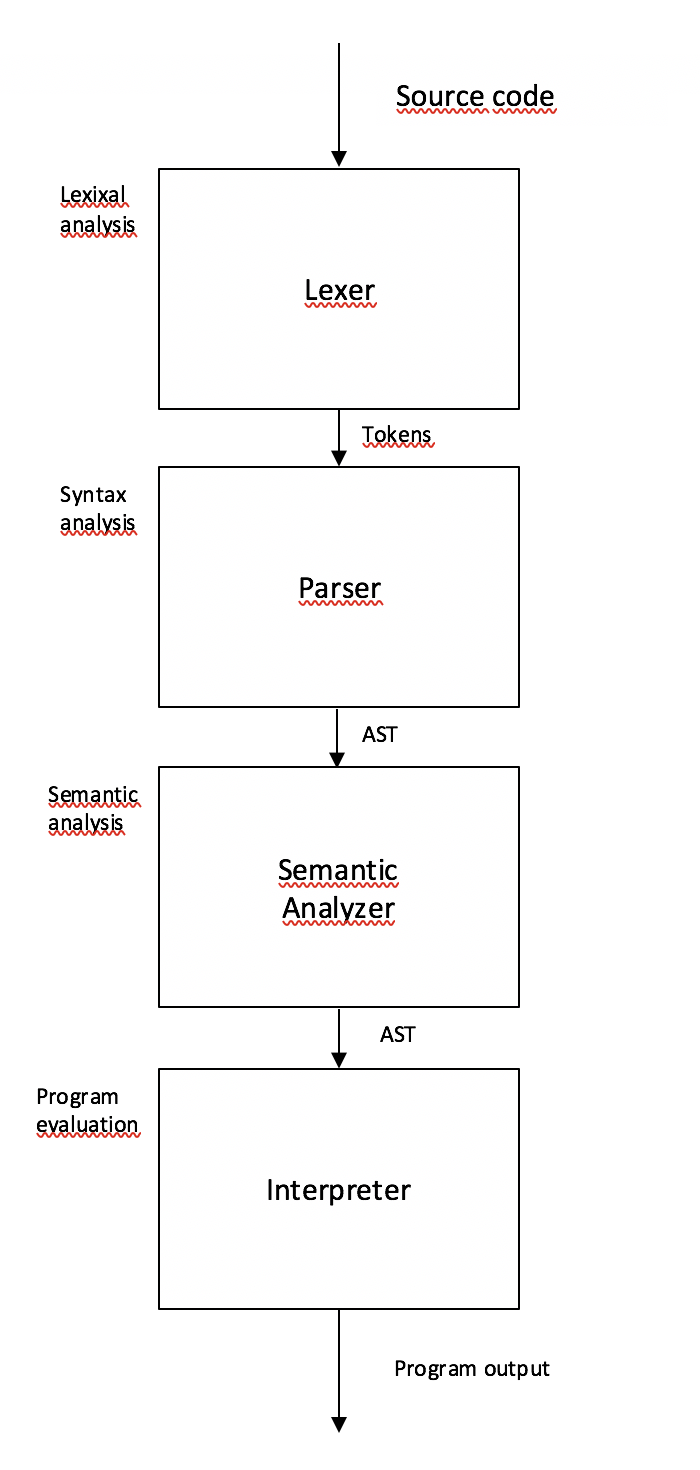
\includegraphics[width=0.4\textwidth]{images/intepreter}}
\caption[intepreter]{Štruktúra interpretera}
\label{obr:intepreter}
\end{figure}

\subsection{Štruktúra interpretera}
Interpreter sa skladá z troch častí: front-end, middle-end a back-end \cite{br3}.

\begin{enumerate}
	\item Front-end (Predná časť) - overuje syntax a sémantiku špecifickú pre daný zdrojový kód. 
	Pokiaľ je program na vstupe syntakticky nesprávny, obsahuje syntaktickú chybu, 
	interpreter by mal vhodným spôsobom na to reagovať. 
	Predná časť spravidla zahŕňa lexikálnu analýzu, syntaktickú analýzu a sémantickú analýzu.
	Výstupom prác prednej časti interpreteru býva program v intermediárnom kóde, 
	ktorý je poskytovaný na spracovanie nasledujúcim častiam interpreteru.

	\item Middle-end (Stredná časť) - vykonáva optimalizácie nad intermediárnym kódom. 
	Tieto optimalizácie sú nezávislé na architektúre cieľového počítača. 
	Príkladom optimalizácií v strednej časti prekladu je odstraňovanie zbytočných 
	alebo nedosiahnuteľných častí kódu, či optimalizácia cyklov. Výstupom tejto časti interpretera 
	je optimalizovaný intermediárny kód, ktorý je následne používaný zadnou časťou interpretera.

	\item Back-end (Zadná časť) -  môže vykonávať dodatočnú analýzu a optimalizácie, 
	ktoré sú špecifické pre cieľový počítač. V každom prípade je však jej hlavnou úlohou 
	generovanie cieľového kódu.
\end{enumerate}

\subsection{Lexikálna analýza, syntaktická analýza a sémantická analýza}

\subsubsection{Lexikálna analýza}
Lexikálna analýza je činnosť, ktorú má na starosť tzv. lexikálny analyzátor - 
je súčasťou prekladača. Lexikálny analyzátor rozdelí vstupnú postupnosť znakov na \textbf{lexémy}. 
Tieto lexémy sú reprezentované vo forme tokenov (symbolov), tie sú poskytnuté 
ku spracovaniu syntaktickému analyzátoru.

\textbf{Lexémy} sú základné symboly programovacieho jazyka, patria sem identifikátory,
kľúčové slová, konštanty rôznych typov, operátory.

\subsubsection{Syntaktická analýza}
Syntaktická analýza sa v informatike nazýva proces analýzy postupnosti 
formálnych prvkov s cieľom určiť ich gramatickú štruktúru voči predom danej formálnej gramatike.
Program, ktorý vykonáva tuto úlohu, sa nazýva syntaktický analyzátor (parser) - 
vstupný text transformuje na určité dátové štruktury, syntaktický strom, 
ktorý zachováva hierarchické usporiadanie vstupných symbolov, ktoré sú vhodné pre ďalšie spracovanie.

\subsubsection{Sémantická analýza}
Sémantická analýza postupne prechádza symboly či skupiny symbolov získané 
zo syntaktickej analýzy a priraďuje sa im význam. Pokiaľ napríklad skupina symbolov
predstavuje použitie konkrétnej premennej, tak analyzátor zisťuje či je premenná už 
deklarována a či je správne použitá  vzhľadom k jej dátovému typu.

\subsection{Syntaktický strom}
Abstraktný syntaktický strom je v informatike stromovou reprezentáciou 
abstraktnej syntaktickej štruktúry zdrojového kódu 
napísaného v programovacom jazyku. 
Abstraktný syntaktický strom sa využíva primárne na preklad a optimalizáciu kódu.

\subsubsection{Štruktúra syntaktického stromu}

\begin{itemize}
	\item vnútorné uzly stromu sú operátory

	\item listy stromu sú jeho operandy

	\item každá časť podstromu je samostatnou logickou jednotkou
\end{itemize}

Nasledujúci obrázok \ref{obr:tree} vychádza z daného kódu
\begin{lstlisting}
	while b != 0:
		if a > b:
			a = a - b
		else:
			b = b - a
	return a
\end{lstlisting}


\begin{figure}[H]
    \centering
    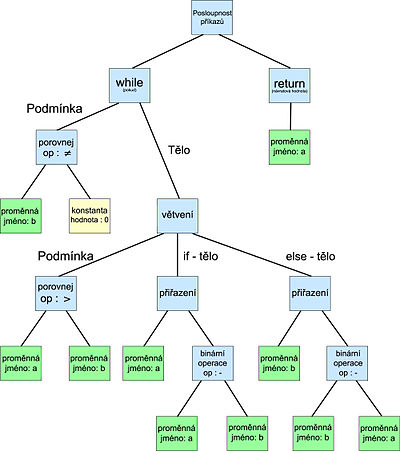
\includegraphics[width=0.4\textwidth]{images/syntakticky_strom}
    \caption[Syntaktický strom]{Syntaktický strom}
    \label{obr:tree}
\end{figure}


\subsection{Model checking}
Overovanie modelov alebo model checking je automatizovaná metóda formálnej verifikácie 
paralelného systému s konečným počtom stavov. Kontroluje sa, či zadaný model vyhovuje špecifikácii. 
Model sa zadáva ako systém prechodov stavov, kde vrcholy sú stavy, a postupnosť prechodov predstavuje
vykonávanie správania sa modelu. Špecifikácia systému sa zadáva formulami temporálnej logiky. 
Výsledkom verifikácie je odpoveď na otázku, či model spĺňa špecifikáciu \cite{br4}.

\subsection{Temporálna logika}  
Tento špeciálny typ logiky je efektívnym nástrojom skúmania procesov v informatike, kde
jednotlivé stavy systému (počítača, programu, atď.) majú časovú následnosť a podmienenosť. 
Kripkeho sémantika pre temporálnu logiku poskytuje transparentnú metódu pre pravdivostné ohodnotenie formúl, 
ktoré špecifikujú stavy informatického systému. Kripkeho model $M = (W, R, v)$ je teraz zjednodušene
špecifikovaný tak, že množina W je nahradená lineárne usporiadanou množinou časových okamžikov 
(bodov) $T = \{t_1, t_2, t_3, ...\}$, pričom $0 \leq t_1 < t_2 < t_3 < ...$ \cite{br10}.

% \subsubsection{Výhody}

% \begin{itemize}
% 	\item Žiadne dôkazy
% 	\item Rýchlosť
% 	\item Kontra príklady
% 	\item Žiadne problémy s čiastočnými špecifikáciami
% 	\item Logika môže vyjadriť veľa súbežných vlastností
% \end{itemize}

% \subsubsection{Nevýhody}

% \begin{itemize}
% 	\item Príliš veľa procesov
% 	\item Dátové cesty
% 	\item Výkonovo náročné
% \end{itemize}

\subsection{CTL*}
CTL* je temporálna logika, ktorá v sebe spája lineárnu časovú logiku LTL a 
logiku výpočtového stromu CTL. Vieme ňou vyjadriť všetko čo dokáže vyjadriť LTL a CTL. Spolu s tým
dokážeme vytvárať formule, ktoré LTL a CTL nedokážu. Avšak zaobchádzať s touto logikou je dosť zložité.
Preto je vhodnejšie pracovať jednotlivo buď s LTL alebo CTL logikou.

\subsubsection{LTL - Linear Time Logic}
Lineárna časová logika LTL rozširuje výrokovú logiku a je reprezentovaná stromom, ktorý má jedinú vetvu.
Táto vetva obsahuje stavy programu, ktoré sú závislé na čase. LTL navyše od výrokovej logiky obsahuje 
aj temporálne operátory ako je napríklad \textbf{X} (ne\textbf{X}t), ktorým sa pýtame na nasledujúci
stav. Medzi ďalšie operátory patrí \textbf{U} (\textbf{U}ntil), \textbf{F} (\textbf{F}innaly) a
\textbf{G} (\textbf{G}lobally) 


\subsubsection{CTL - Computation Tree Logic}
Je logika, ktorá pracuje na úrovni stromov, ktorá dokáže zabezpečiť aby niečo platilo vo všetkých 
stavoch alebo existuje aspoň jeden stav, pre ktorý to platí. K tomu nám pomáhajú kvantifikátory 
$\forall$ a $\exists$. Pomocou spojenia týchto kvanfikátorov a temporálnych operátorov z LTL 
nám vznikne CTL - logika výpočtového stromu. Takýto strom sa skladá zo stavov a hrán, ktoré vedú k
ďalším stavom. Počet stavov a teda úrovní daného stromu je nekonečný. Jednotlivé kombinácie kvantifikovaných
a temporálnych operátorov môžeme vidieť na obrázkoch \ref{obr:AF}, \ref{obr:AG}, \ref{obr:EF} a \ref{obr:EG}.


\begin{figure}[H]
	\centering
	\begin{minipage}{.5\textwidth}
	  \centering
	  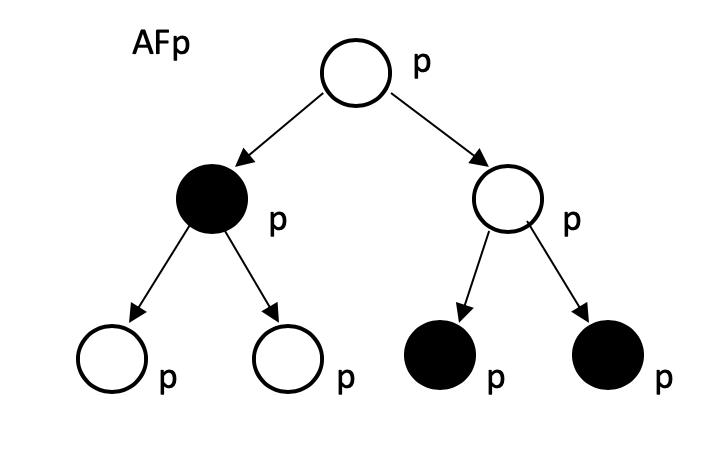
\includegraphics[width=1\linewidth]{images/AF}
	  \caption[Formula AFp]{Formula AFp}
	  \label{obr:AF}
	\end{minipage}%
	\begin{minipage}{.5\textwidth}
	  \centering
	  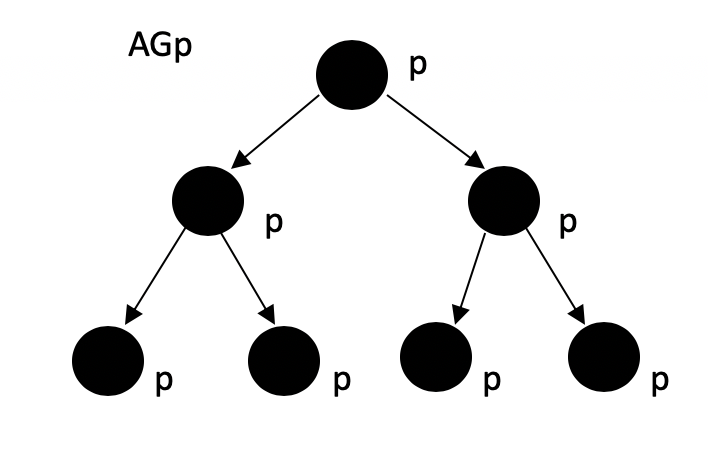
\includegraphics[width=.95\linewidth]{images/AG}
	  \caption[Formula AGp]{Formula AGp}
	  \label{obr:AG}
	\end{minipage}
\end{figure}

\begin{figure}[H]
	\centering
	\begin{minipage}{.5\textwidth}
	  \centering
	  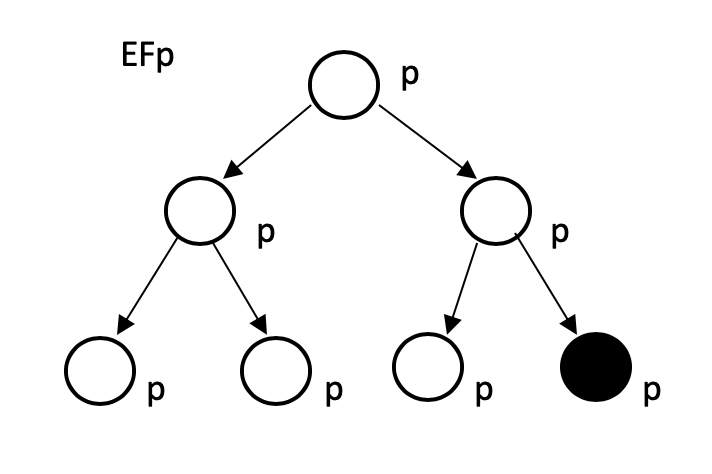
\includegraphics[width=1\linewidth]{images/EF}
	  \caption[Formula EFp]{Formula EFp}
	  \label{obr:EF}
	\end{minipage}%
	\begin{minipage}{.5\textwidth}
	  \centering
	  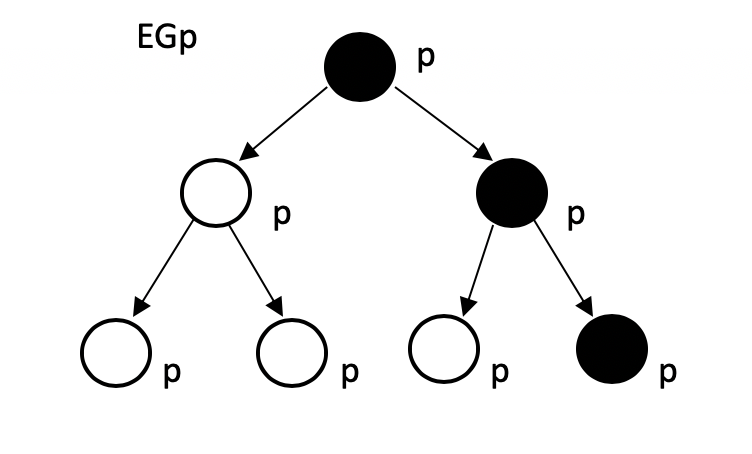
\includegraphics[width=1.1\linewidth]{images/EG}
	  \caption[Formula EGp]{Formula EGp}
	  \label{obr:EG}
	\end{minipage}
\end{figure}


\subsection{LTSmin}
LTSmin (model checker) začal ako všeobecná sada nástrojov na manipuláciu s označenými prechodovými systémami. 
Medzitým bola sada nástrojov rozšírená na plný overovací model, 
pri zachovaní jeho jazykovo nezávislých charakteristík.

Na získanie svojho vstupu LTSmin spája značný počet existujúcich overovacích 
nástrojov: muCRL , mCRL2 , DiVinE , SPIN (SpinS), UPPAAL (opaal), SCOOP , PNML , ProB a CADP.

LTSmin má modulárnu architektúru, ktorá umožňuje prepojenie viacerých front-end modelovacích 
jazykov s rôznymi analytickými algoritmami prostredníctvom spoločného rozhrania.
Poskytuje symbolické aj explicitné algoritmy analýzy viacerých jazykov, 
ktoré umožňujú viaceré spôsoby riešenia problémov pri konflikte.
Toto prepojovacie rozhranie sa nazýva Partitioned Next-State Interface (PINS, obr. \ref{obr:pins}), 
ktorého základom je definícia stavového vektora, počiatočný stav, 
funkcia NextState a funkcie označovania \cite{br5}.

\begin{figure}[H]
\centerline{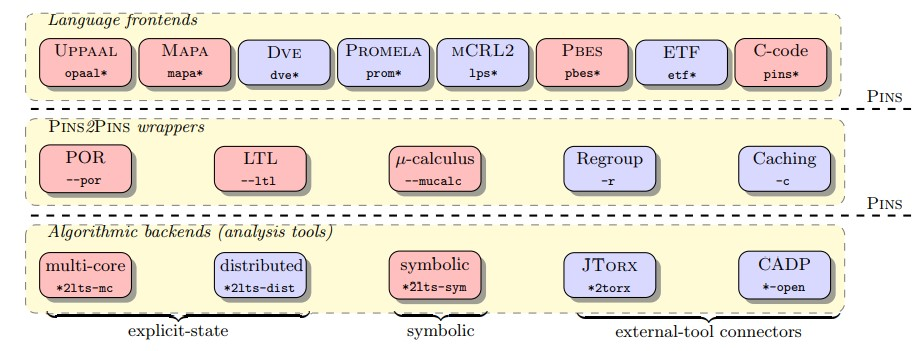
\includegraphics[width=1\textwidth]{images/ltsmin}}
\caption[PINS architektúra (obrázok bol prevzatý zo zdroja \cite{br5})]{PINS architektúra (obrázok bol prevzatý zo zdroja \cite{br5})}
\label{obr:pins}
\end{figure}

\subsubsection{Back-ends}
LTSmin ponúka rôzne analytické algoritmy zahŕňajúce tri algoritmické backendy:

\begin{itemize}
	\item Distribuované inštancie
	\item Viacjadrový model
	\item Symbolická kontrola modelu
\end{itemize}

\subsubsection{Front-ends}
LTSmin už spája značný počet existujúcich overovacích nástrojov ako jazykových modulov, 
čo umožňuje používať ich modelové formalizmy:

\begin{itemize}
	\item muCRL
	\item mCRL2
	\item DiVinE
	\item SpinS
	\item UPPAAL
	\item SCOOP
	\item PNML
	\item ProB
	\item CADP
\end{itemize}

\subsubsection{PINS2PINS}
Rozhranie PINS čisto rozdeľuje naše kontrolné nástroje do dvoch nezávislých častí: 
\begin{itemize}
	\item jazykové moduly
	\item algoritmy kontroly modelov
\end{itemize}
Umožňuje však aj vytvorenie modulov PINS2PINS (obr. \ref{obr:pins2pins}), 
ktoré sa nachádzajú medzi jazykovým modulom a algoritmom.
Tieto moduly PINS2PINS môžu využívať všetky algoritmické backendy a 
môžu byť zapnuté a vypnuté na požiadanie:

\begin{itemize}
	\item Transition caching do vyrovnávacej pamäte zvyšuje pomalé jazykové moduly
	\item Regrouping urýchľuje symbolické algoritmy pomocou optimalizácie závislostí
	\item Partial-order znižuje stavový priestor tým, že klesne irelevantné prechody
\end{itemize}

\begin{figure}[H]
\centerline{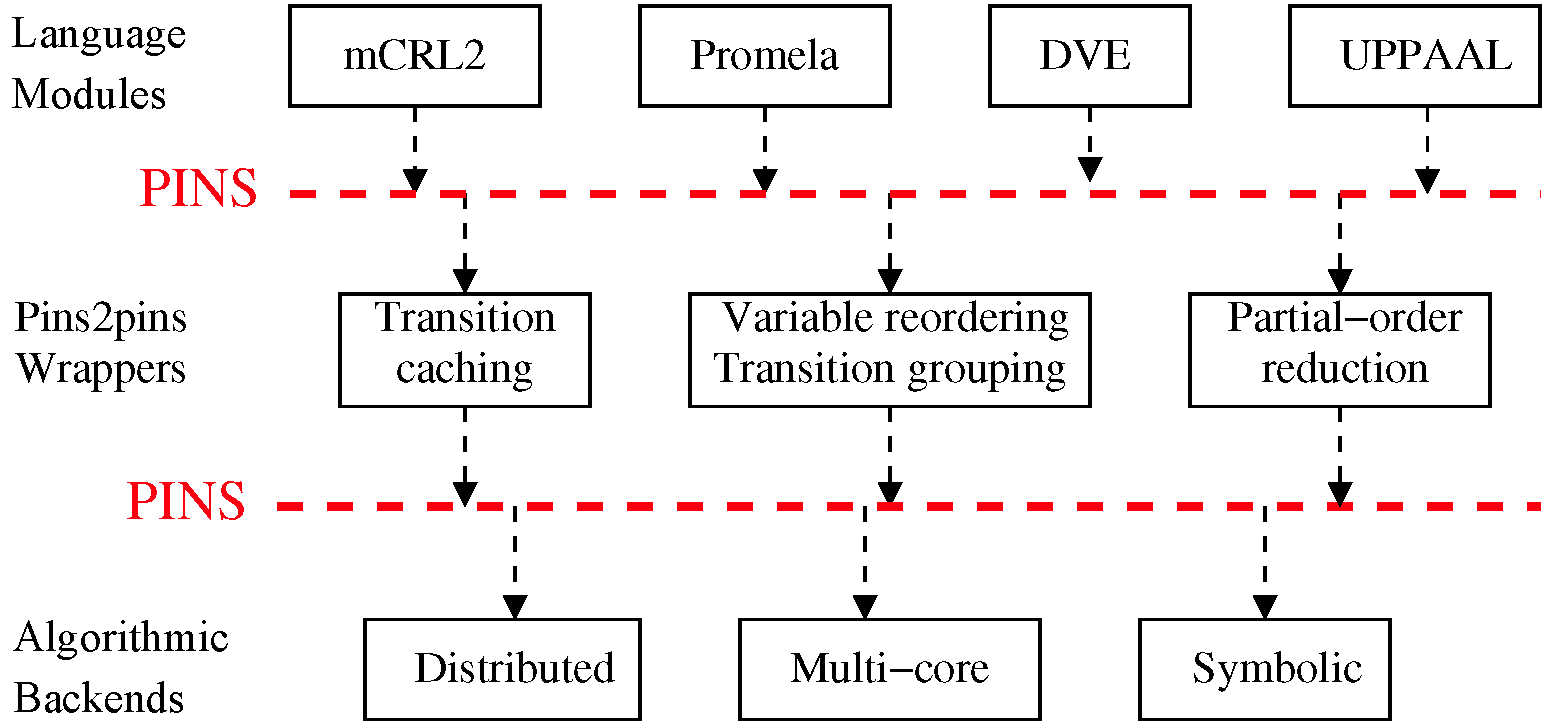
\includegraphics[width=0.7\textwidth]{images/pins2pins}}
\caption[PINS2PINS (obrázok bol prevzatý zo zdroja \cite{br5})]{PINS2PINS (obrázok bol prevzatý zo zdroja \cite{br5})}
\label{obr:pins2pins}
\end{figure}